% what is shown in the GUI
% what is the difference between the two subject groups
% what information is saved
%
\section{Visual Feedback}
This section provides information on how the visual feedback was presented to the subjects in the to experiment groups.

\begin{figure}[H] 
\centering
	\begin{subfigure}[b]{0.3\textwidth}
		\centering
		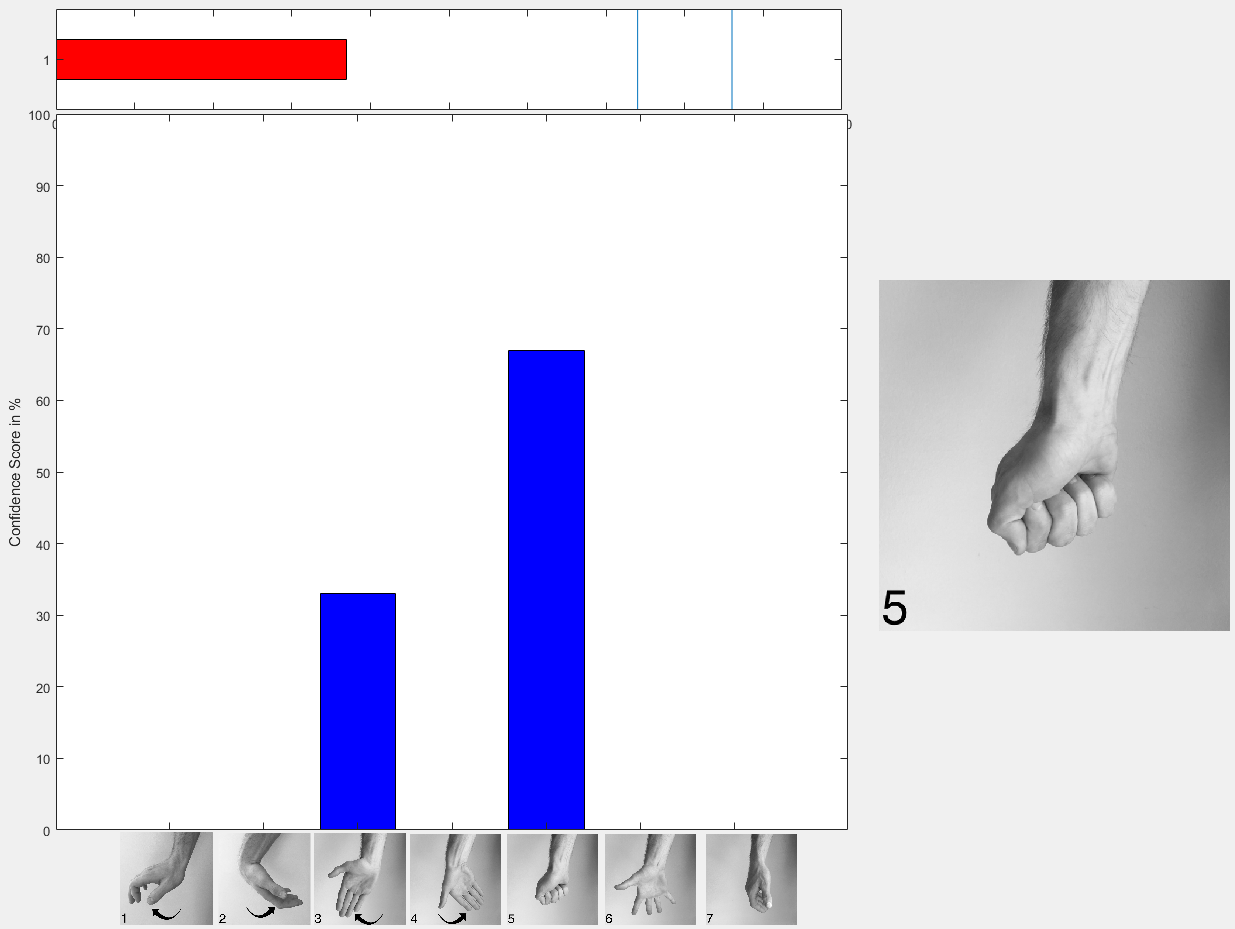
\includegraphics[width=.4\textwidth]{figures/xBackground/usertraintestGUI}  
		\caption{Illustration of the user training interface for the test group showing the bar plot indicating the confidence level of movement recognition and horizontal bar plot indicating contraction level. The picture on the right side of the bar plot indicates which movement needs to be performed.}
	\end{subfigure}                
	\begin{subfigure}[b]{0.3\textwidth}
		\centering
		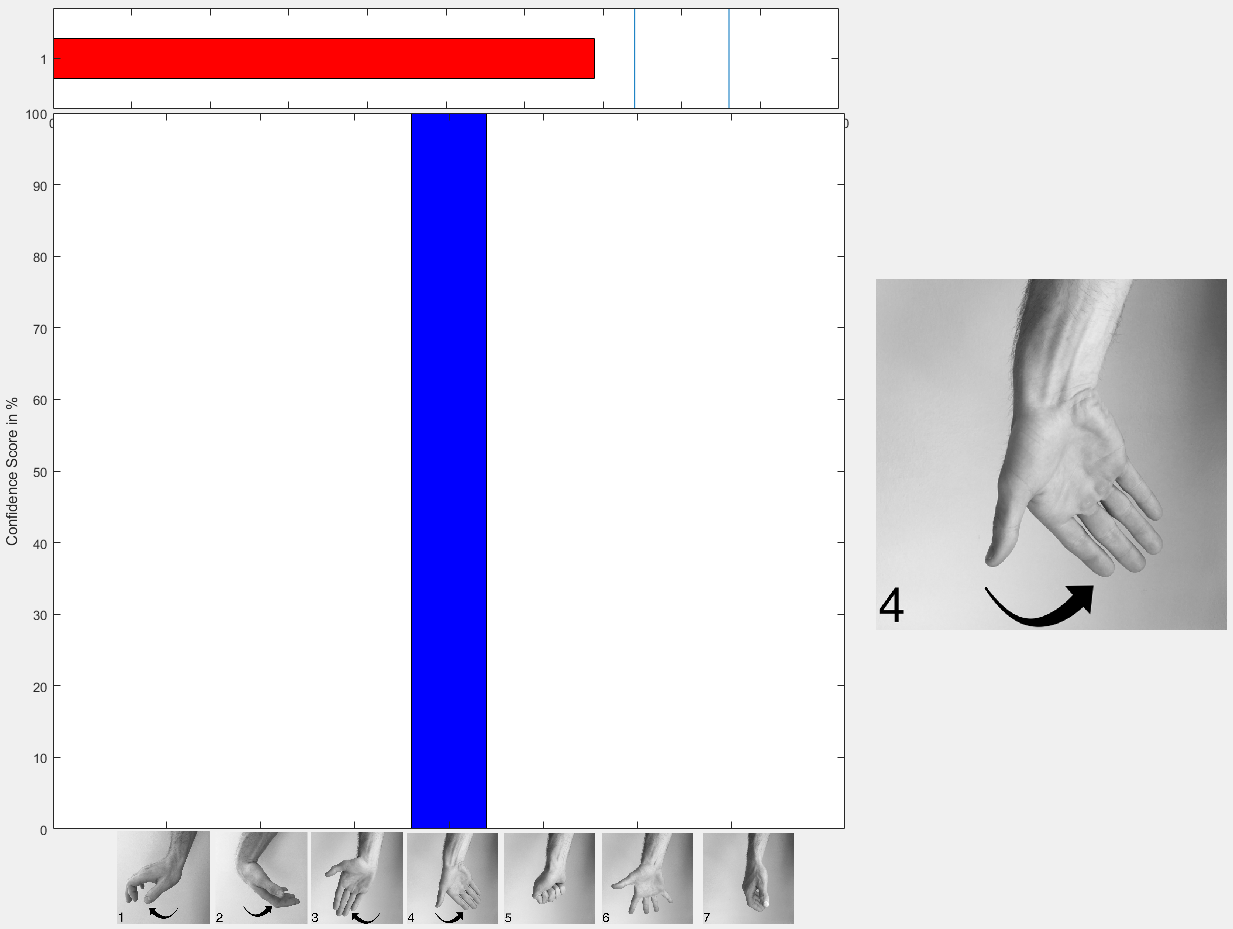
\includegraphics[width=.4\textwidth]{figures/xBackground/usertraincontrolGUI}  
		\caption{Illustration of the user training interface for the control group showing the bar plot indicating which movement is being recognized and the horizontal bar plot indicating contraction level. The picture on the right side of the bar plot indicates which movement needs to be performed.}
	\end{subfigure}
	\caption{A figure with two subfigures}
    \label{fig:feedbackGUI}
\end{figure}

%\begin{figure}[H]
%	{
%		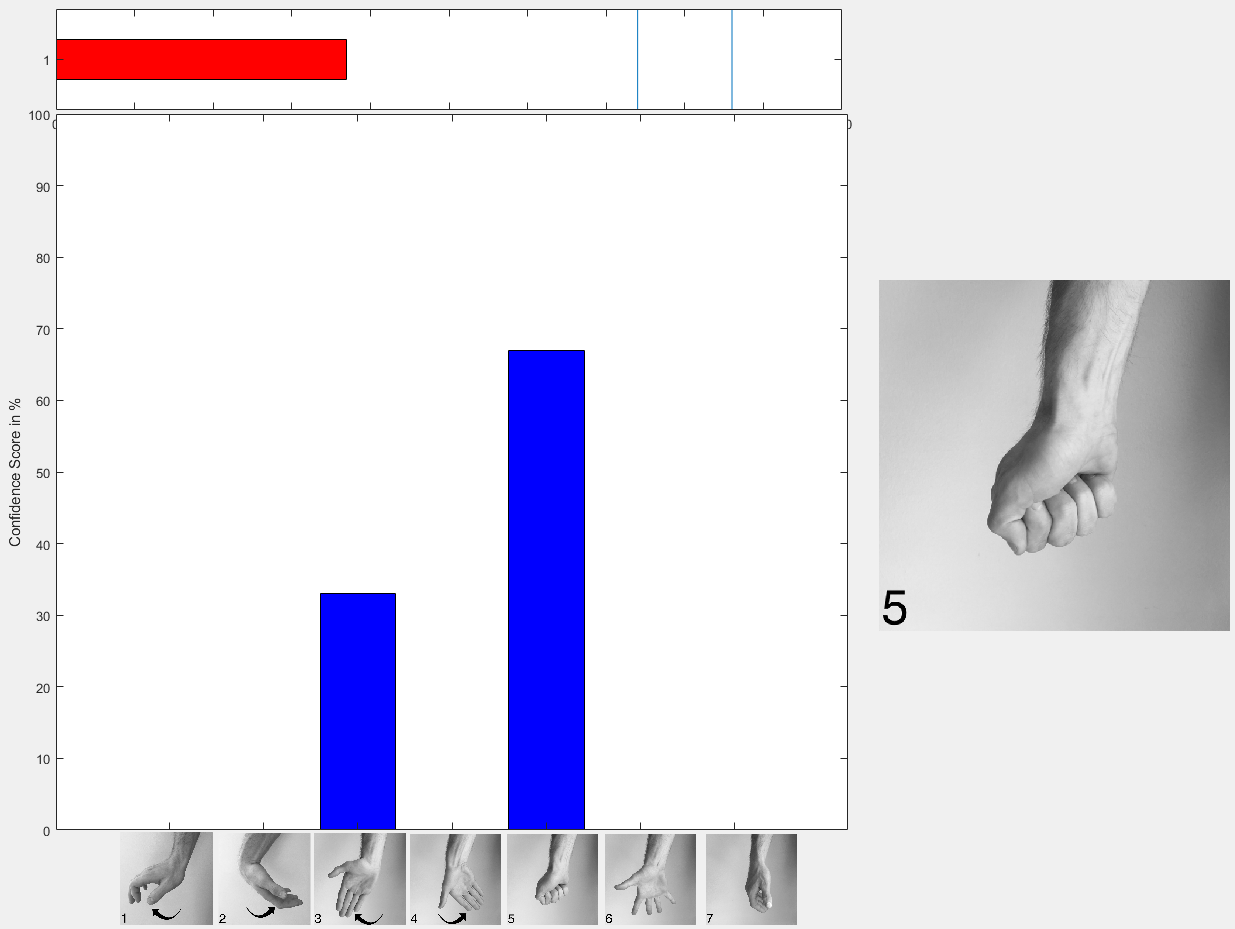
\includegraphics[width=.46\textwidth]{figures/xBackground/usertraintestGUI}
%	}
%	\hspace{5pt}
%	{
%		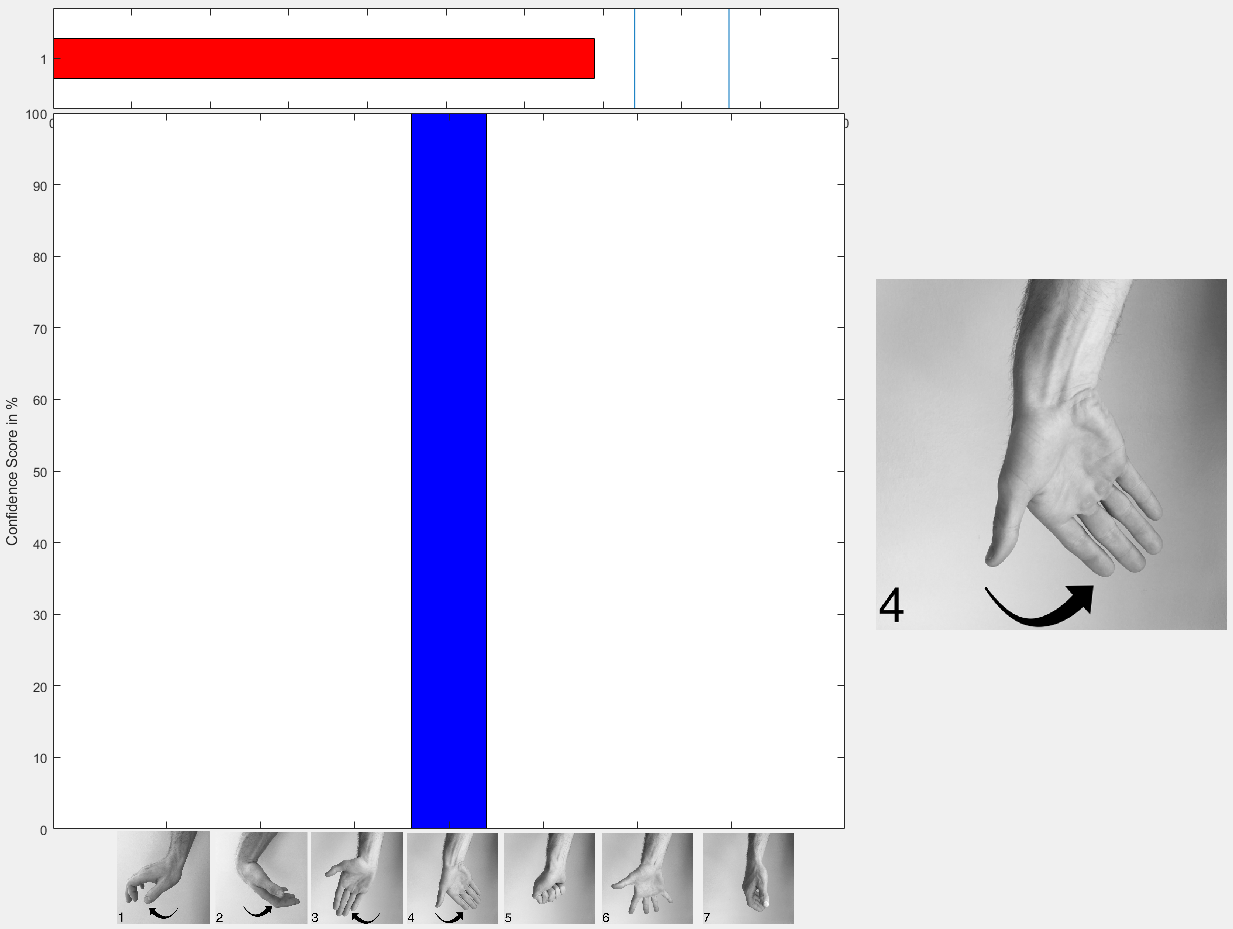
\includegraphics[width=.46\textwidth]{figures/xBackground/usertraincontrolGUI}         
%	}
%	\caption{Illustration of the user training interface for the test group (on the left) and the control group (on the right). showing the bar plot indicating which movement is being recognized and the horizontal bar plot indicating contraction level. The picture on the right side of the bar plot indicates which movement needs to be performed.}
%	\label{fig:feedbackGUI}
%\end{figure}
